\section{Die Web Content Class Definition Language}
    \label{section:solutionDetailsDSL}
    Begonnen wird mit der \gls{wccdl} --
    der domänenspezifischen Sprache zur Definition von Klassen.
    Dazu sind einige Vorkenntnisse über \glspl{dsl} im Allgemeinen
    und über die verwendete Language Workbench Xtext erforderlich.
    Diese Grundlagen werden deshalb in diesem Kapitel vermittelt,
    bevor die \gls{wccdl} im Fokus steht.
    Deren Beschreibung orientiert sicht an Völters u.a.
    \cite{voelter:DslEngineering}
    allgemeinen Design Dimensionen und Paradigmen von \glspl{dsl}.

    \subsection{Domänenspezifische Sprachen}
    Domänenspezifische Sprachen (engl. Domain specific languages (DSLs))
    sind spezielle Sprachen zum Ausdrücken der Programme einer speziellen
    Problemdomäne \cite[Kapitel 2.2]{voelter:DslEngineering}.

    Im Gegensatz zu \glspl{gpl} sind \glspl{dsl} nicht zwangsläufig Turing-Vollständig
    und deshalb nicht generell austauschbar.
    Stattdessen ist eine \gls{dsl} spezialisiert und optimiert auf eine gegebene Domäne,
    weshalb sie eng mit deren Konzepten und Abstraktionen verbunden ist
    und in Form von speziellen Sprachkonzepten wiederspiegelt.
    Technische und unnötige Details blendet sie aus und überträgt diese Verantwortung
    auf die Execution Engine, d.h. einen Interpreter oder einer Repräsentation in einer
    niedrigeren Sprache, zu der sie transformiert wird.
    Dadurch kann eine \gls{dsl} die Programme ihrer Domäne kürzer und mit einer besseren Semantik
    als \glspl{gpl} ausdrücken \cite[Kapitel 2.2]{voelter:DslEngineering}.

    Durch die Verwendung einer \gls{dsl} steigert sich sowohl die Produktivität
    als auch die Qualität des Ergebnisses,
    da der Entwickler sich stärker auf die eigentliche Problemstellung und weniger
    auf unterstützende technische Aspekte konzentrieren kann.
    Der Quelltext wird dadurch bei gleichbleibender Semantik kürzer und besser les- sowie wartbar.
    Dies wird auch durch die eingeschränkten Möglichkeiten des Entwicklers,
    durch die er weniger Fehler produzieren kann, unterstützt.
    Die stärkere Semantik erleichtert die Implementierung von Analysen und die Formulierung
    hilfreicher Fehlermeldungen.
    Sowohl der Bau als auch Verwendung einer \gls{dsl} fördert das Verständnis der Domäne
    der Entwickler, steigert die Kommunikation und erlaubt die Einbeziehung von Domänenexperten
    \cite[Kapitel 2.5]{voelter:DslEngineering}.
    Aspekte, die auch in \citet{evans:DomainDrivenDesign} Domain Driven Design eine zentrale Rolle spielen.

    \glspl{dsl} sind natürlich auch mit einigen Herausforderungen verbunden.
    Dazu zählt zunächst der zusätzliche Aufwand, der durch den Entwurf und Bau einer \gls{dsl} entsteht,
    der durch moderne Werkzeuge allerdings verringert werden kann.
    Gleichzeitig erfordert der Entwurf einer guten Sprache Erfahrung,
    da die Domäne nicht nur analysiert und modelliert werden muss,
    sondern auch entschieden werden muss, welche Konzepte in welcher Form in die Sprache übernommen werden.
    Iterative Vorgehen sind hierbei zu empfehlen.
    Die Implementierung einer oftmals nur schwer portiert werden,
    wodurch eine Abhängigkeit zum verwendet Werkzeug entsteht.
    Nicht zuletzt müssen die Nutzer der Sprache diese erlernen,
    was ebenfalls Aufwand erzeugt.
    Gleichzeitig kann sich das parallele Lernen der Domäne und der Sprache positiv auf einander auswirken
    \cite[Kapitel 2.6]{voelter:DslEngineering}.

    \glspl{dsl} sollten generell nicht eingesetzt werden,
    wenn ein kein gemeinsames Verständnis der Domäne und keine Möglichkeit dieses zu erlangen
    existiert.
    Außerdem sollte die Erfahrung der Entwickler in diesem Bereich ausreichend sein,
    um erfolgreich zu sein.

    Eine Umsetzung einer \gls{dsl} kann generell in zwei Formen geschehen:
    Als "`Internal \gls{dsl}"' oder als "`External \gls{dsl}"'.
    Internal \glspl{dsl} nutzen die Sprachmöglichkeiten einer anderen Sprache
    -- meist einer \gls{gpl} --, wodurch sie sich in diese einbetten und
    Programme schnell den Eindruck machen eine ganz neue Sprache zu verwenden.
    Technisch stellen sie aber nur eine geschickte Nutzung der Sprachmöglichkeiten
    einer anderen Sprache, kombiniert mit einigen die Domäne modellierenden Programmierschnittstellen, dar.
    Sie besitzen keinen eigenen Compiler oder Interpreter und stellen deshalb immer gültige Programme
    in der Wirtssprache dar.
    Ihr Vorteil ist ihre vergleichsweise leichte Umsetzung sowie die Möglichkeit das Umfeld der Sprache,
    wie Standardbibliotheken leicht nutzen zu können
    \cite[Kapitel 2.8.1]{voelter:DslEngineering}.

    External \glspl{dsl} stellen hingegen komplett eigenständige Programmiersprachen dar,
    bei denen der Syntax komplett frei definierbar ist,
    wodurch die Domäne oftmals simpler wiedergespiegelt werden kann.
    Sie erfordern allerdings mehr Aufwand, zum Beispiel bei der Definition der Grammatik
    und der Implementierung eines Generators oder Interpreters.

    Bei der entwickelten Sprache handelt es sich um eine externe \gls{dsl}.
    \subsection{Xtext}
    \label{section:solutionDetailsDslXtext}
    Xtext ist ein Framework zur Entwicklung von \glspl{dsl} und ihrer Integration
    in die Entwicklungsumgebung Eclipse\footnote{\url{https://www.eclipse.org/}}.
    Dies beinhaltet die automatische Generierung eines Parsers,
    das Bauen und Speichern des abstrakten Syntaxbaumes eines Programmes,
    Hilfsmittel zum Schreiben eines Code-Generators oder Interpreters
    sowie eine automatische Umsetzung gängiger Funktionen von
    Entwicklungsumgebungen, wie Quelltexthervorhebung und Autovervollständigung
    \cite[Kapitel 1]{bettini:xtext}.
    Zur Erweiterung und Anpassung dieser Artefakte ist die Sprache Xtend vorgesehen.
    Dabei handelt es sich um eine Java-ähnliche \gls{gpl},
    die zusätzliche Sprachmittel bietet, wie zum Beispiel Typinferenz.
    Sie wurde als Proof-of-Concept selbst mit Xtext entwickelt
    \cite[Kapitel 3]{bettini:xtext}.
    Die Entwicklung einer \gls{dsl} mit Xtext erfordert lediglich die Definition
    einer Grammatik, auf dessen Basis das Framework unter anderem die genannten 
    Artefakte generiert.
    Regeln in dieser Grammatik werden über Anweisungen definiert,
    die der erweiterten Backus-Naur-Form ähneln.
    Zur Generierung eines Parsers setzt Xtext auf
    ANTLR\footnote{vgl. \url{http://www.antlr.org/}},
    welches einen LL(*)-Algorithmus implementiert
    \cite{xtext:documentation,parr:antlr}.

    \subsection{Sprachkonzepte}
    \label{solutionDetails:dslConcepts}
    Die \gls{wccdl} spiegelt die Konzepte aus
    Kapitel \ref{section:conceptClassesFeaturesSelectors}
    durch Linguistic Abstractions wider.
    Die folgende Beschreibung orientiert sich an den
    Domänenkonzepten.
    
    \paragraph*{Klassen}
    Abbildung \ref{image:dslClasses} modelliert,
    wie das Konzept der Klassen in der \gls{wccdl} abgebildet wird.

    \begin{figure}[htb]
        \centering
        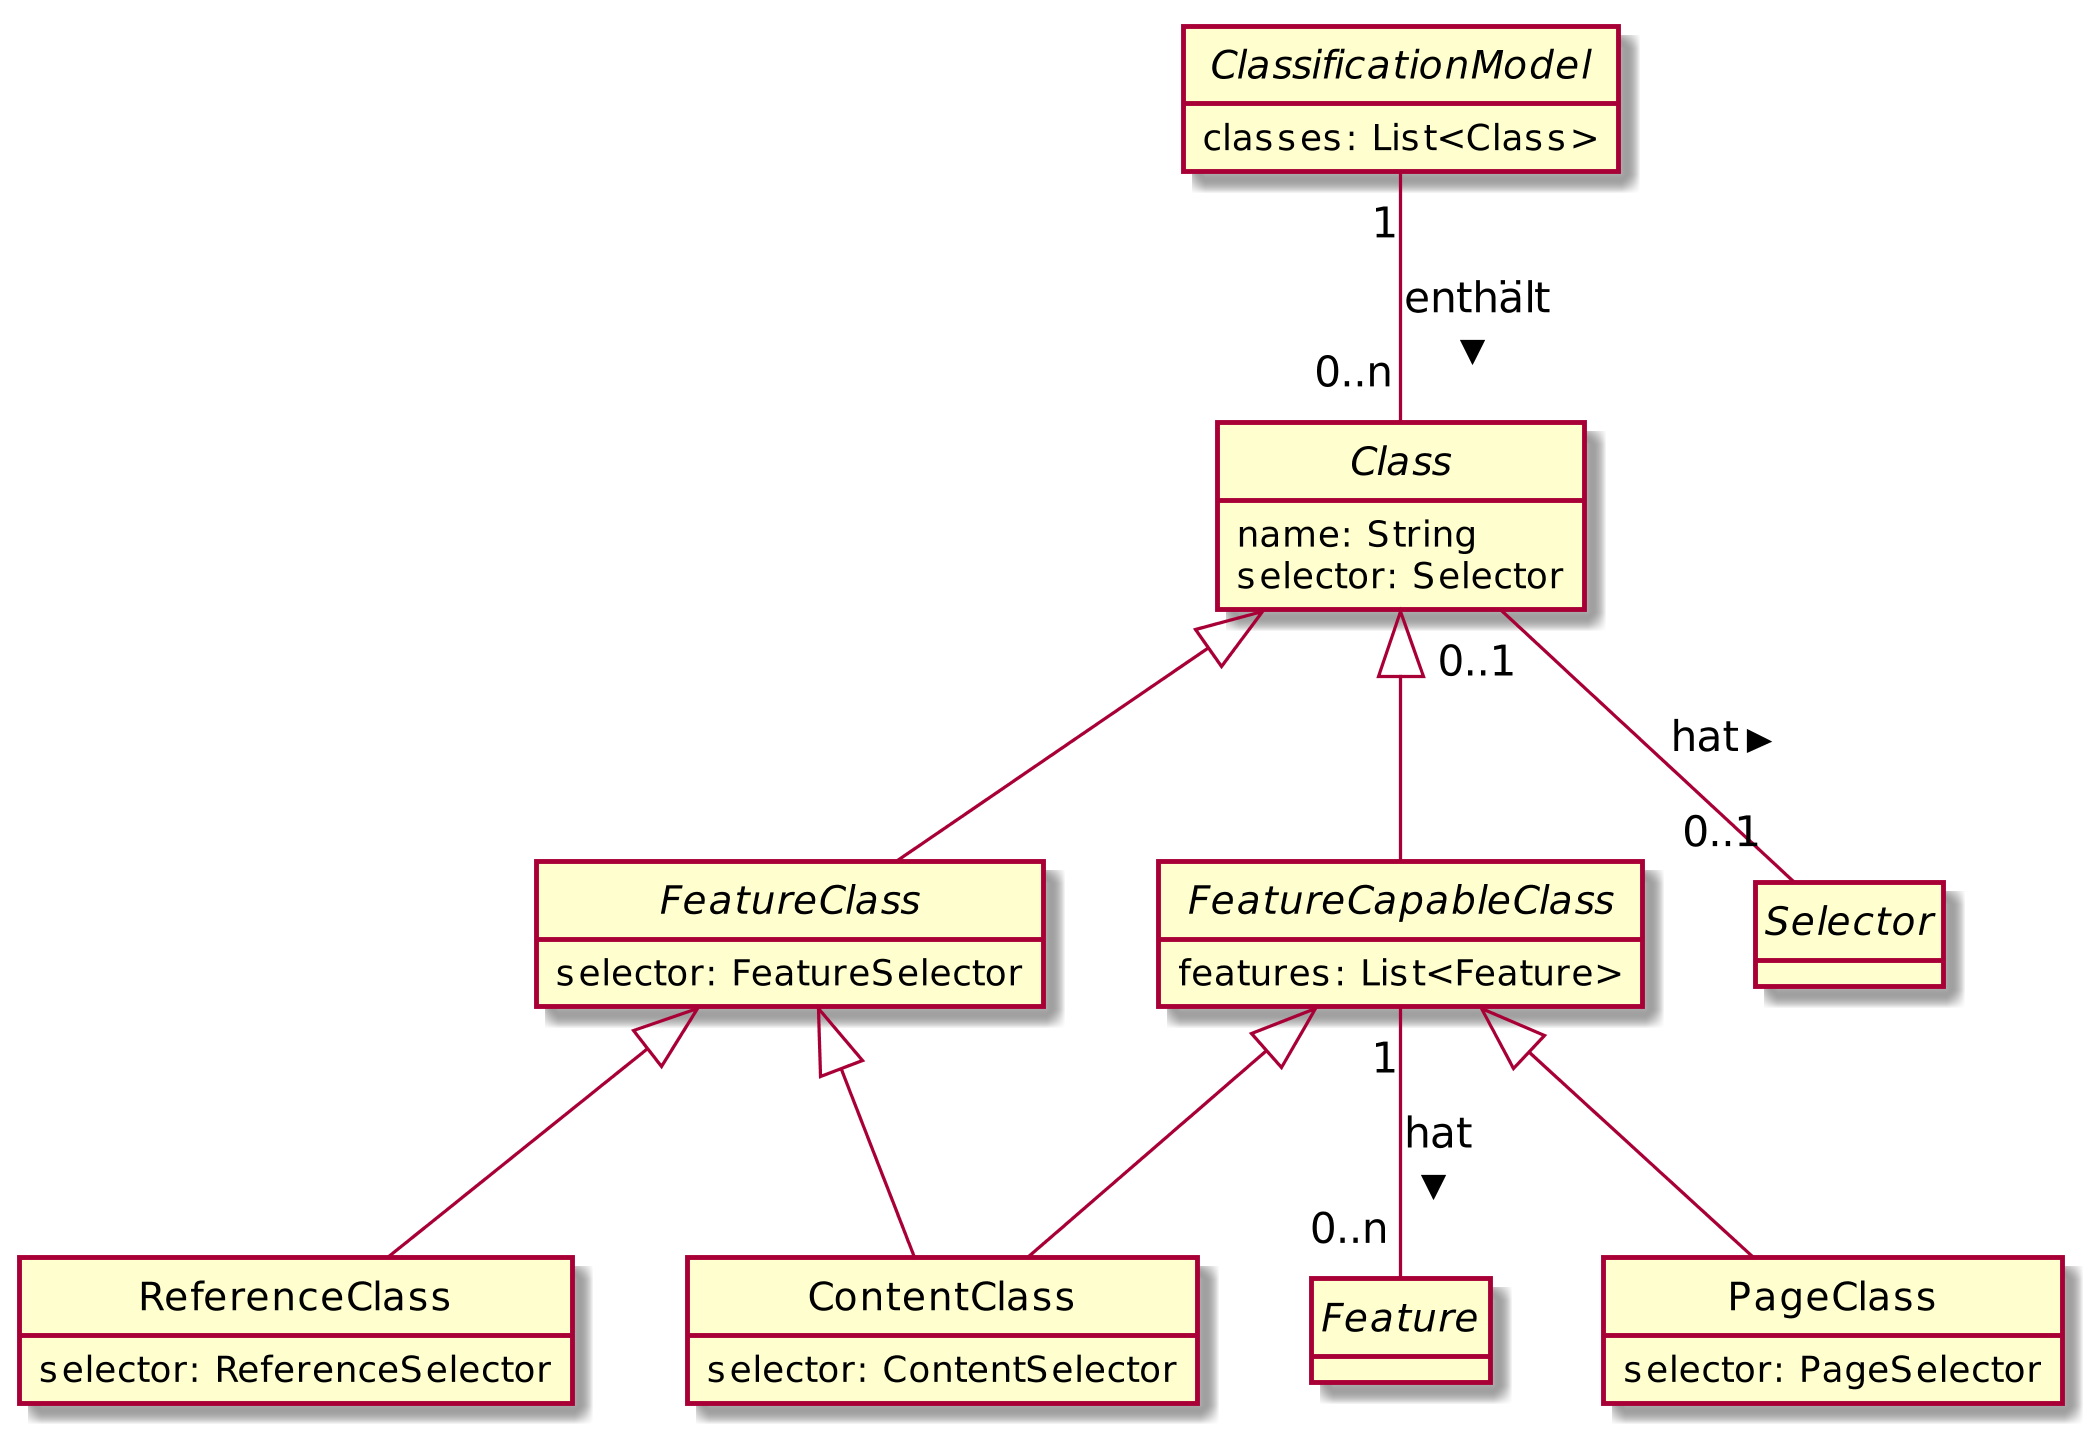
\includegraphics[scale=\imageScalingFactor]{../resources/dsl/classes.png}
        \caption{Klassen in der \acrshort{wccdl}}
        \label{image:dslClasses}
    \end{figure}

    Zentraler Bestandteil der Sprache ist das abstrakte Konzept \texttt{Class},
    welches gemäß der Domänenkonzepte in drei konkrete Ausprägungen unterteilt wird:
    \texttt{PageClass}, \texttt{ContentClass} und \texttt{ReferenceClass}.
    Jedes in der \gls{wccdl} geschriebene Programm ist eine Sammlung
    von Klassendefinitionen und enthält deshalb genau ein \texttt{ClassificationModel},
    das wiedrum beliebig viele Instanzen der genannten Konzepte beinhalten kann.
    Klassen besitzen einen Namen und einen Selektor,
    der -- ausgenommen von Seitenklassen -- optional ist.
    Die Sprache enthält hierzu das entsprechende Konzept \texttt{Selector},
    welches weiter unten vorgestellt wird.
    Da nicht jeder Selektor für jede Klasse geeignet ist,
    verwenden die einzelnen Klassentypen verschiedene Selektortypen,
    wobei es sich um \texttt{PageSelector}, \texttt{ContentSelector}
    und \texttt{ReferenceSelector} handelt,
    die ebenfalls später genauer thematisiert werden.
    Wieso der Selektor Teil der Typinformation von \texttt{ContentClass}
    und \texttt{ReferenceClass} ist,
    wird bei der unteren Diskussion der Features ersichtlich.
    Lediglich Seiten- und Inhaltsklassen können Features besitzen,
    weshalb die Sprache das Konzept \texttt{FeatureCapableClass} einführt,
    um diese Eigenschaft auszudrücken.
    \texttt{PageClass} und \texttt{ContentClass} sind
    Ableitungen dieses Konzeptes, welches
    wiederum eine Spezialisierung von \texttt{Class} ist.
    Auf der anderen Seite sind nur Inhalts- und Referenzklassen als Klasse eines Features geeignet.
    Für diese Eigenschaft enthält die Sprache das Konzept \texttt{FeatureClass},
    welches ebenfalls von \texttt{Class} erbt und
    von dem sowohl \texttt{ContentClass} als auch \texttt{ReferenceClass} ableiten.

    \paragraph*{Features}
    Die \gls{wccdl} repräsentiert Features über das gleichnamige Sprachkonzept,
    was Abbildung \ref{image:dslFeatures} veranschaulicht.
    Analog zum Domänenkonzept besitzt jedes Feature in der Sprache einen Namen
    und eine Klasse, welche vom oben vorgestellten Typ \texttt{FeatureClass} sein muss.
    Des Weiteren kann ein Feature einen Selektor besitzen,
    um den der Klasse für sich zu überschreiben.
    Da nicht jede Selektorart für Features geeignet ist,
    führt die Sprache das Konzept \texttt{FeatureSelector} ein,
    um eine Unterscheidung zwischen geeigneten und ungeeigneten Arten möglich zu machen.
    Auf \texttt{FeatureSelector} wird weiter unten genauer eingegangen.
    In Bezug auf den Selektor eines Features ist außerdem relevant,
    ob dieser für die Klasse des Features geeignet ist.
    Das heißt, ob der Selektor zum Beispiel ein \texttt{ContentSelector} ist,
    wenn es sich bei der Klasse um eine Inhaltsklasse handelt.
    Dies wird sichergestellt,
    indem der Typ des Selektors Teil der Typinformation von
    \texttt{Feature} ist und sowohl die Eigenschaften \texttt{class} als auch
    \texttt{selector} diesen verwenden und damit zueinanderpassen müssen.
    Ob es sich bei einem Feature um ein {\scalarFeature} oder ein {\collectionFeature} handelt,
    ist aus Sicht der Sprache lediglich eine boolesche Eigenschaft und erfordert
    keine weitere Unterscheidung.
    Das ist eine Abweichung vom Modell des Domänenkonzeptes, die dadurch begründet ist,
    dass die Sprache Features lediglich deklariert und nicht sicherstellen muss,
    dass in einer konkreten Klassifikation alle Elemente eines {\collectionFeature}s die gleiche Klasse verwenden.
    Eine Unterscheidung zwischen {\contentFeature}s und {\referenceFeature}s
    ist ebenfalls nicht notwendig,
    da diese Information klar aus der verwendeten \texttt{FeatureClass} hervorgeht.

    \begin{figure}[tb]
        \centering
        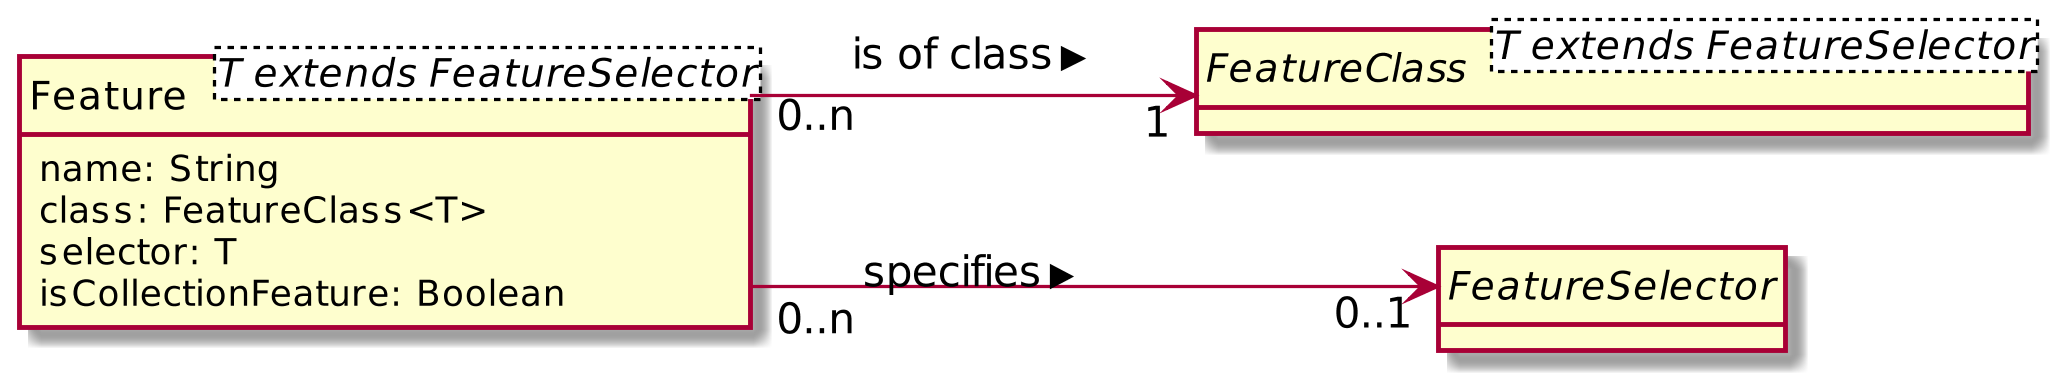
\includegraphics[scale=\imageScalingFactor]{../resources/dsl/features.png}
        \caption{Features in der \acrshort{wccdl}}
        \label{image:dslFeatures}
    \end{figure}

    \paragraph*{Selektoren}
    Die \gls{wccdl} bietet des Weiteren Konzepte zur Definition von Selektoren,
    die vereinzelt schon angesprochen wurden.
    Eine vollständige Übersicht bietet Abbildung \ref{image:dslSelectors}.

    \begin{figure}[htb]
        \centering
        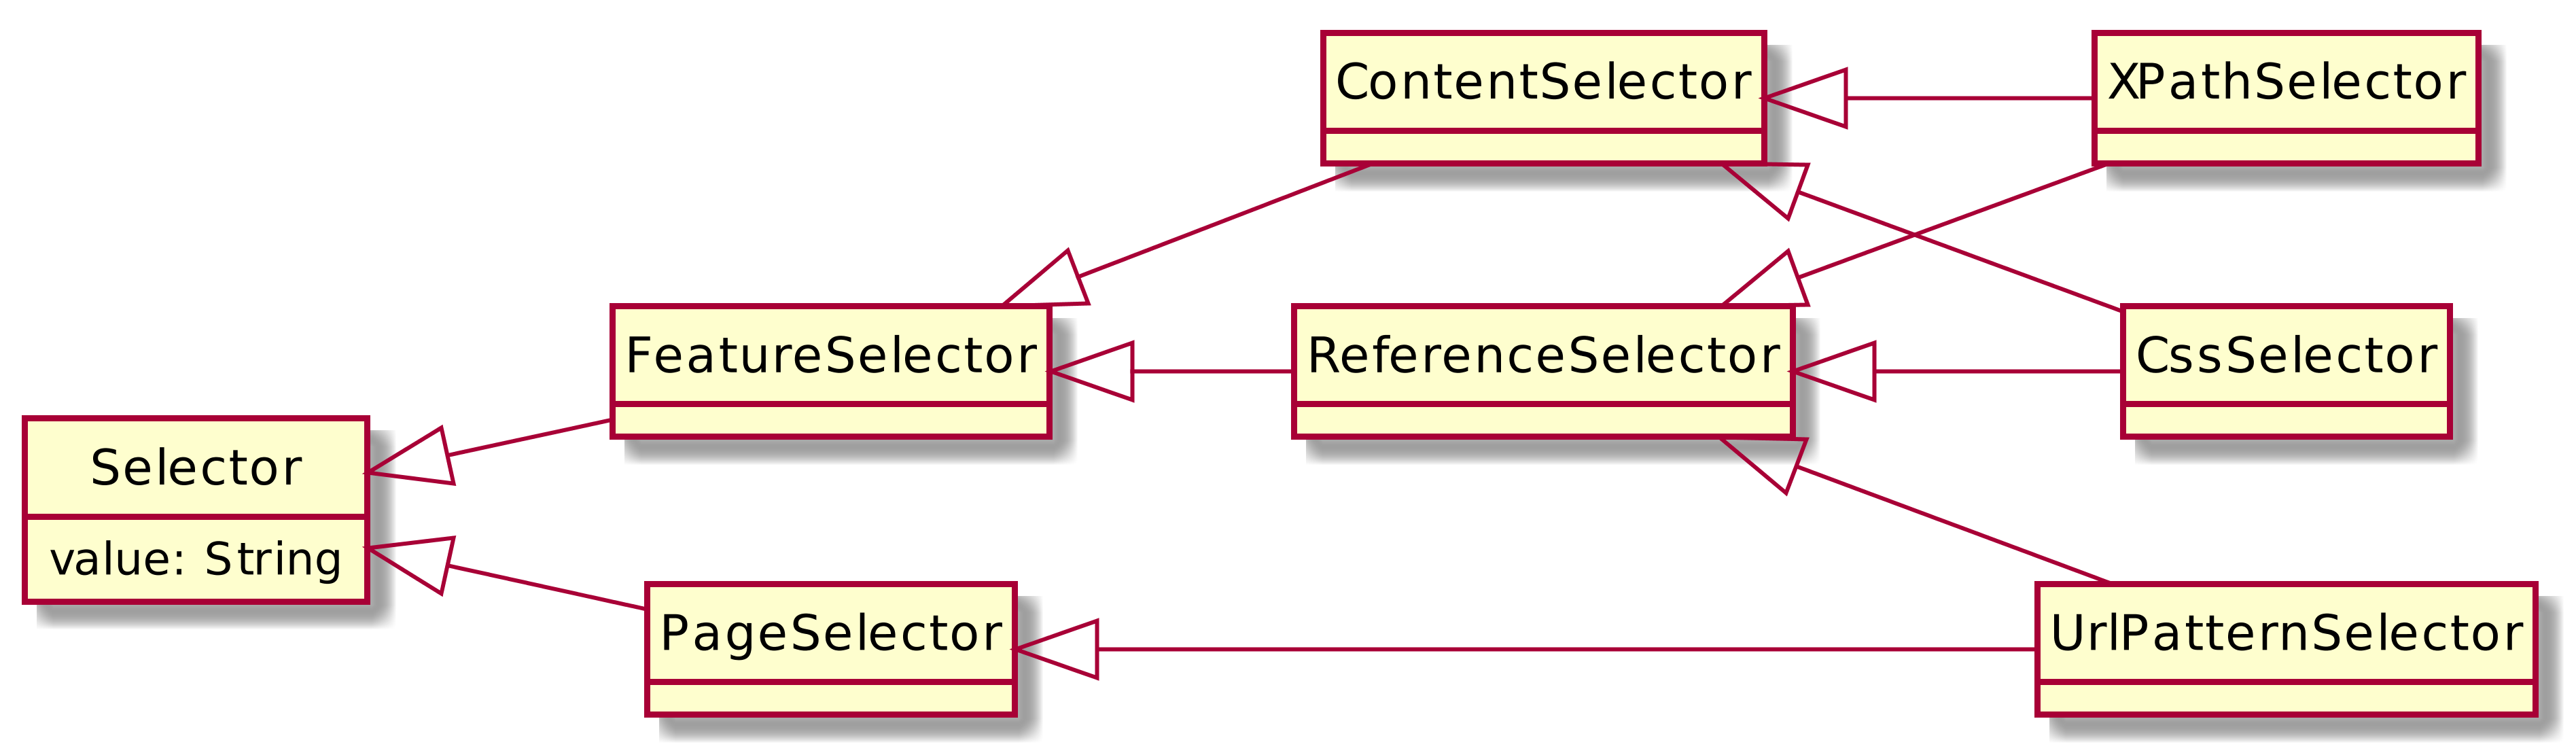
\includegraphics[scale=\imageScalingFactor]{../resources/dsl/selectors.png}
        \caption{Selektoren in der WCML}
        \label{image:dslSelectors}
    \end{figure}

    Das abstrakte Konzept \texttt{Selector} entspricht dem gleichnamigen Domänenkonzept
    und unterteilt sich in weitere abstrakte Konzepte,
    mit denen Selektoren nach ihrer Eignung für die verschiedenen Klassentypen getrennt werden.
    Diese Konzepte sind \texttt{PageSelector}, \texttt{ContentSelector} und \texttt{ReferenceSelector}.
    Die vom Klassifizierungssystem unterstützten
    Selektoren\footnote{vgl. Kapitel \ref{section:conceptSupportedSelectors}}
    spiegelt die \gls{wccdl} mit den konkreten Konzepten
    \texttt{CssSelector}, \texttt{XPathSelector} und \texttt{UrlPatternSelector} wider,
    die die zuvor genannten Konzepte spezialisieren.
    Dadurch wird eindeutig abgebildet, welche Selektorarten für welche Klassentypen geeignet sind.
    Ein weiterer relevanter Aspekt ist die Eignung der Selektoren für Features,
    wozu das bereits erwähnte Konzept \texttt{FeatureSelector} existiert.
    Da Features nur Inhalts- oder Referenzklassen verwenden können,
    leiten nur \texttt{ContentSelector} und \texttt{ReferenceSelector} von diesem ab.
    
    \subsection{Strukturelles Design}
    Dieses Kapitel beschreibt einige strukturelle Aspekte der \gls{wccdl},
    die im Wesentlichen auf den Ausführungen in \cite[Kapitel 4 \& 5.1]{voelter:DslEngineering}
    basieren.

    \paragraph*{Separation of Concerns}
    Eine Domäne kann aus verschiedenen Aspekten bestehen,
    die verschiedene Bereiche der Domäne abdecken.
    Alle diese Belange müssen beim Design der Sprache berücksichtigt werden.
    \citet[Kapitel 4.1]{voelter:DslEngineering}
    stellen dazu zwei Ansätze vor: Eine Sprache, die alle Aspekte adressiert
    und mehrere Sprachen, die sich auf jeweils einen Aspekt fokussieren.
    Für den Anwendungsfall der \gls{wccdl} lassen sich die
    folgenden Aspekte identifizieren:

    \begin{enumerate}
        \item Die Deklaration von Klassen, d. h. sie lediglich bekannt zu machen.
        \item Die Definition von Klassen, d. h. die Angabe von Features.
        \item Die Definition von Selektoren für Klassen und Features.
    \end{enumerate}

    Wie aus den bisherigen Ausführungen bereits deutlich wurde,
    deckt die \gls{wccdl} alle diese Aspekte ab,
    da sie sehr eng gekoppelt sind und jeweils einen sehr geringen Umfang besitzen.

    \paragraph*{Modularisierung und Sichtbarkeit}
    Die Modularisierung beschreibt die logische Strukturierung
    von Programmelementen und wird durch jede Sprache in irgendeiner Form adressiert.
    Ein Beispiel ist die Strukturierung der Elemente in Namensräume.
    Die Referenzierung eines Elementes sollte immer auf der logischen
    Struktur erfolgen, weshalb die Modularisierung eng mit der Sichtbarkeit
    von Programmelementen verbunden ist.
    Auch dieses Konzept ist in jeder Sprache vertreten und legt fest,
    von wo ein Element referenziert werden kann
    \cite[Kapitel 5.1.1]{voelter:DslEngineering}.
    In Java lässt sich dieser Raum z. B. über die Schlüsselwörter
    \texttt{private} und \texttt{protected} einschränken
    \cite[Kapitel 6.6]{oracle:javaSpec}.
    Die \gls{wccdl} verwendet ein sehr einfaches Konzept bez.
    der Modularisierung und Sichtbarkeit von Programmelementen.
    Klassen sind die einzigen Elemente, die in dieser Sprache das Ziel einer Referenz
    sein können, weshalb Features und Selektoren implizit nirgendwo sichtbar sind.
    Klassen werden in einem globalen Modul gesammelt und sind überall sichtbar,
    sodass sie für jedes Feature genutzt werden können.

    \paragraph*{Partitionierung}
    Die Strukturierung eines Programmes in physische Einheiten (Dateien) heißt Partitionierung.
    Da die Referenzierung von Programmelementen nur auf Basis der logischen Struktur erfolgen sollte,
    muss die physische der logischen Strukturierung nicht entsprechen
    \cite[Kapitel 5.1.2]{voelter:DslEngineering}.
    Die \gls{wccdl} erlaubt die Klassendefinitionen auf verschiedenen Dateien
    aufzuteilen, wobei eine Klasse immer vollständig in einer Datei enthalten sein muss.
    Da alle Klassen logisch in einem globalen Namensraum gesammelt werden,
    sind auch Klassen anderer Dateien referenzierbar.

    \paragraph*{Scoping und Linking}
    Der Scope eines Querverweises in einem Programm ist die Menge der
    gültigen Ziele dieser Referenz.
    Linking beschreibt den Transformationsprozess vom syntaktischen Baum des Programmes
    zum semantischen Graphen, bei dem Verweise basierend auf den Namen der referenzierten
    Elemente aufgelöst werden
    \cite[Kapitel 8]{voelter:DslEngineering}.
    Querverweise sind in der \gls{wccdl} nur zur Angabe der Klasse eines Features notwendig.
    Der Scope wird an dieser Stelle bereits durch das Sprachkonzept hinreichend
    eingeschränkt, da das Ziel vom Typ
    \texttt{FeatureClass} sein muss.
    Das Linking wird vollständig durch Xtext übernommen
    \cite[Kapitel "`Language Implementation"']{xtext:documentation}.

    \paragraph*{Spezifikation und Implementierung}
    Sprachen können die Trennung von Spezifikation und Implementierung von
    Programmelementen unterstützen, um eine bessere Entkopplung und verschiedene
    Implementierungen zu ermöglichen \cite[Kapitel 5.1.3]{voelter:DslEngineering}.
    Ein Beispiel aus Java sind Interfaces \cite[Kapitel 9]{oracle:javaSpec}.
    Eine denkbare Anwendung dieser Idee in der \gls{wccdl} ist Selektoren als
    Implementierung zu betrachten. Dann könnte man Klassen inkl. Features einmalig spezifizieren
    und z. B. für verschiedene Sites durch verschiedene Selektoren unterschiedlich "`implementieren"'.
    Die \gls{wccdl} unterstützt eine solche Trennung bisher allerdings nicht.

    \paragraph*{Spezialisierung}
    In vielen Sprachen können Programmelemente andere erweitern und somit eine Spezialisierung formulieren.
    In diesen Fällen erbt das konkrete Element alle Eigenschaften des allgemeinen
    und kann deshalb an dessen Stelle verwendet werden
    \cite[Kapitel 5.1.4]{voelter:DslEngineering}.
    Für die \gls{wccdl} wäre dieses Konzept für Klassen denkbar,
    um ihre Selektoren, Features und deren Selektoren zu vererben.
    Sie unterstützt diese Funktion bisher allerdings nicht.

    \paragraph*{Typen und Instanzen}
    Die in einer Programmiersprache definierten Typen können bei ihrer Instanziierung
    häufig Parameter entgegennehmen, wodurch sich ihre Wiederverwendbarkeit steigert.
    Ein Beispiel sind die Parameter eines Konstruktors in objektorientierten Programmiersprachen
    \cite[Kapitel 5.1.5]{voelter:DslEngineering}.
    In der \gls{wccdl} können Features den Selektor ihrer Klasse überschreiben,
    was eine Anwendung dieses Konzeptes ist.

    \paragraph*{Superposition und Aspekte}
    \citet[Kapitel 5.1.6]{voelter:DslEngineering} beschreiben zwei
    allgemeine Sprachkonzepte, durch die Programmfragmente zusammengeführt
    oder verändert werden können.
    Superposition vereint mehrere Fragmente anhand eines speziellen Operators.
    Aspekte bieten die Möglichkeit, durch eine Abfrage verschiedene Codestellen
    auszuwählen und aspektspezifisch zu modifizieren.
    Die \gls{wccdl} unterstützt keines dieser Konzepte,
    da sie für ihren Anwendungsfall zu komplex sind und kein sinnvoller Anwendungsfall existiert.

    \paragraph*{Sprachmodularität}
    Dieses Konzept beschreibt die Möglichkeit (Teil-)Sprachen wiederzuverwenden
    und zu einer neuen zusammenzusetzen.
    Dadurch kann Konsistenz gewahrt und eine doppelte Implementierung vermieden werden.
    Die verschiedenen Ansätze die \citet[Kapitel 4.6]{voelter:DslEngineering} beschreiben
    sind Language Referencing, Extension, Reuse und Embedding.
    Für die \gls{wccdl} bietet sich die Einbettung anderer Sprachen zur Definition von Selektoren an,
    um Entwickler bei der Formulierung von CSS-, XPath und regulären Ausdrücken zu unterstützen
    und die syntaktische Korrektheit von Selektoren sicherzustellen.
    Bisher setzt die Sprache dies aber nicht um.

    \subsection{Statische Semantik}
    \label{section:solutionDetailsDslStaticSemantics}
    Die statische Semantik einer Sprache beschreibt alle Bedingungen,
    die zum Zeitpunkt der Kompilierung eines Programmes erfüllt sein müssen.
    \citet[Kapitel 4.3]{voelter:DslEngineering} unterteilen sie in die Kategorien
    Constraints und Type System Rules.
    Die \gls{wccdl} besitzt kein komplexes Typsystem,
    da an keiner Stelle Typen berechnet werden müssen.
    Ein Großteil der typbezogenen Bedingungen wird stattdessen über
    Sprachkonzepte
    sichergestellt.
    Allerdings gibt es einige Bedingungen, die so nicht gewährleistet werden können.
    Hierfür implementiert die Sprache folgende semantische Validierungen:

    \begin{enumerate}
        \item Der Name einer Klasse ist global eindeutig.
        \item Der Name eines Features ist lokal (innerhalb ihrer Klasse) eindeutig.
        \item   Falls die Klasse eines Features keinen Selektor spezifiziert,
                definiert das Feature einen Selektor.
        \item   Falls ein Feature einen Selektor spezifiziert,
                ist dieser mit der Klasse des Features kompatibel.
        \item Der Wert eines Selektors ist nicht leer und besteht nicht ausschließlich aus Leerzeichen.
    \end{enumerate}

    \subsection{Dynamische Semantik}
    Die dynamische Semantik eines Programmes beschreibt das Verhalten
    während der Laufzeit. Deshalb wird sie auch als "`Execution Semantics"' bezeichnet
    \cite[Kapitel 4.3]{voelter:DslEngineering}.
    Die \gls{wccdl} ist eine rein deklarative Sprache.
    Sie beschreibt keinen Kontrollfluss sondern lediglich
    Klassen, deren Features und Selektoren.
    Wie diese Informationen verarbeitet werden, ist für die Sprache unerheblich.
    Deshalb wird der Programmcode nicht in ein ausführbares Programm übersetzt,
    sondern in ein anderes Format transformiert.
    Bezüglich des Laufzeitverhaltens trägt die \gls{wccdl}
    deshalb lediglich die Verantwortung, ein {\classificationModel}
    semantisch äquivalent in dieses Format zu übersetzen.
    \subsection{Generierung}
    \label{section:solutionDetailsDslGeneration}
    Ein {\classificationModel} wird in ein JSON-Dokument übersetzt,
    wozu ein entsprechender Generator implementiert wurde.

    \paragraph{Klassen}
    Im generierten Zustand werden die Klassendefinitionen weiterhin nach
    Seiten-, Inhalts- und Referenzklassen unterteilt,
    was im JSON-Dokument durch die Schlüssel \texttt{pageClasses},
    \texttt{contentClasses} und \texttt{referenceClasses} geschieht.
    Ihre Objekte enthalten wiederum Schlüssel-Wert-Paare,
    wobei der Schlüssel in diesem Fall der Name einer Klasse und der
    Wert die Klasse selbst ist.
    Klasse speichern ihren Namen zusätzlich in der Eigenschaft \texttt{name},
    sodass sie auch ohne Kontext identifizierbar sind.
    Listing \ref{listing:dlsGenerationPageClass} zeigt dies am Beispiel
    der Seitenklasse \texttt{Service}.
    Inhalts- und Referenzklassen sind sehr ähnlich aufgebaut.

    \lstinputlisting[
        label=listing:dlsGenerationPageClass,
        caption=Ein Beispiel einer Seitenklasse in einem generierten {\classificationModel},
        style=json
    ]{../resources/dsl/generation/page-class.json}

    \paragraph{Selektoren}
    Unter \texttt{selector} ist in Listing \ref{listing:dlsGenerationPageClass}
    der Selektor der Klasse gespeichert,
    was seinen Typ und seinen Wert umfasst.
    Der Selektor einer Klasse ist niemals undefiniert,
    kann im Falle von Inhtals- oder Referenzklassen aber ein leeres Objekt sein.
    Dann ist der Selektor von den Features zu beziehen.
    Der Typ eines Selektors ist immer \texttt{CssSelector},
    \texttt{UrlPatternSelector} oder \texttt{XPathSelector}.
    Im Beispiel ist zu sehen, dass der {\urlSelector} \verb+\/service\/?$+ codiert wurde.
    Andernfalls würden JSON-Parser z. B. die Rückwärtsschrägstriche als besondere Zeichen interpretieren.
    Der JSON-Standard \cite[Kapitel 7]{rfc:8259} spezifiziert einige Zeichen,
    die innerhalb von Zeichenketten so codiert werden müssen.
    Diese Aufgabe übernimmt der entwickelte Generator,
    sodass Nutzer der \gls{wccdl} sich darum nicht kümmern müssen.
    Eine Ausnahme ist allerdings der {\xpathSelector}.
    XPath 1.0 kennt keine Codierung für besondere Zeichen,
    wie z. B. \texttt{\textbackslash{n}} für einen Zeilenumbruch.
    Außerdem ist in dieser Version die Funktion
    \texttt{codepoints-to-string} noch nicht enthalten,
    mit der Unicode Codes in Zeichenketten umgewandelt werden können
    \cite{w3c:xpath}
    \cite[Kapitel 5.2.1]{w3c:xpathXquery}.
    Um trotzdem Inhalte mit besonderen Zeichen beschreiben zu können,
    wird in {\xpathSelector}en der Rückwärtsschrägstrich während der
    Generierung nicht codiert.
    Das heißt, die Sequenz \texttt{\textbackslash{n}} wird genau so in das JSON-Dokument übernommen.
    Ein JSON-Parser setzt das Zeichen zu einem Zeilenumbruch um,
    wodurch der XPath-Ausdruck einen tatsächlichen Umbruch enthält
    der als solcher interpretiert wird.
    Ein konkretes Anwendungsbeispiel für diese Ausnahme im Generator
    ist im ersten Fallbeispiel in Kapitel \ref{section:findingsTeachersClassificationModel} zu sehen.

    \paragraph{Features}
    Seiten- und Inhaltsklassen können in den Eigenschaften
    \texttt{contents} und \texttt{references} Features speichern.
    Die Struktur eines generierten Features zeigt Listing
    \ref{listing:dlsGenerationFeature} am Beispiel des {\contentFeature}s \texttt{pageHeading}.

    \lstinputlisting[
        label=listing:dlsGenerationFeature,
        caption=Ein Beispiel eines Features in einem generierten {\classificationModel},
        style=json
    ]{../resources/dsl/generation/page-heading-feature.json}

    Wie schon bei Klassen wird der Name des Features sowohl als Schlüssel des Objektes
    als auch innerhalb des Objektes selbst verwendet.
    Außerdem besitzt ein Feature die Eigenschaft \texttt{class},
    die den Namen der Klasse des Features speichert. Dabei handelt es sich immer
    um den Namen einer Klasse aus \texttt{contentClasses} oder \texttt{referenceClasses}.
    Das JSON-Dokument ist also in sich geschlossen.
    Darüber hinaus besitzt jedes Feature die Eigenschaft \texttt{isCollection},
    die entweder \texttt{true} oder \texttt{false} sein kann.
    Sie definiert,
    ob es sich um ein {\scalarFeature} oder ein {\collectionFeature} handelt.
    Wie Klassen enthält auch ein Feature einen Selektor.
    Ist dieser leer, ist der Selektor der Klasse zu verwenden.
    {\childFeature}s werden innerhalb eines Features ebenfalls unter \texttt{contens} bzw.
    \texttt{references} abgelegt.
    \subsection{Konkrete Syntax und deren Grammatik}
    \lstinputlisting[
        label=listing:dlsExample,
        caption=Beispielhafte Klassendeklaration,
        language=wccdl,
        inputencoding=utf8/latin1]{../resources/dsl/example.wccd}    
    \lstinputlisting[
        label=listing:dlsGrammarClasses,
        caption=Klassen in der Grammatik der DSL,
        language=wccdl,
        inputencoding=utf8/latin1]{../resources/dsl/grammar/classes.xtext}
    \lstinputlisting[
        label=listing:dlsGrammarSelectors,
        caption=Selektoren in der Grammatik der DSL,
        language=wccdl,
        inputencoding=utf8/latin1]{../resources/dsl/grammar/selectors.xtext}
    \lstinputlisting[
        label=listing:dlsGrammarFeatures,
        caption=Features in der Grammatik der DSL,
        language=wccdl,
        inputencoding=utf8/latin1]{../resources/dsl/grammar/features.xtext}
    \subsection{Integration in Eclipse}
    Die Nutzung einer Programmiersprache wird durch eine gute Integration in eine
    Entwicklungsumgebung effektiver.
    \citet[Kapitel 12.]{voelter:DslEngineering} zählen eine Reihe von
    Funktionen auf, die solche Werkzeuge bieten können.
    Dazu zählen bspw. die Autovervollständigung und farbliche Hervorhebung von Quelltext
    sowie Refaktorisierungsfunktionen.
    Für viele dieser Mittel generiert Xtext eine Integration
    in die Entwicklungsumgebung Eclipse,
    die bei Bedarf erweitert werden kann\footnote{vgl. Kapitel \ref{section:solutionDetailsDslXtext}}.

    Diese Möglichkeit wurde genutzt, um Selektoren farblich im Editor hervorzuheben.
    Des Weiteren wurde die Autovervollständigung für die Klammern um Selektoren ergänzt,
    da sie auf vielen Tastaturlayouts nicht vorhanden sind.
    Eine dritte Ergänzung sind sprechende Fehlermeldungen für die implementierten
    semantischen Validierungen\footnote{vgl. Kapitel \ref{section:solutionDetailsDslStaticSemantics}}.
    % TODO: Ggf. Screenshots

